\chapter{Deep Learning}
\label{chap: deeplearning}
\begin{chapquote}{\kaishu 《射雕英雄传》}
可怜未老头先白,春波碧草,晓寒深处,相对浴红衣
\end{chapquote}

\section{Model architecture}
\label{sec:ma}
\begin{itemize}
\item How many hidden units should be used? 
\begin{itemize}
    \item Suppose the inputs are M-dimensional, there are D units in the hidden layer. 
    \item If D $>$ M, it's mapping inputs to a higher dimensional space, just the usage of kernel in SVM. 
    \item If D $<$ M, it's a kind of (nonlinear) dimension reduction.
    \item D $=$ 1 and it's the final output, it's simply a logistic regression. 
\end{itemize}
\item How many layers should be used?
\begin{itemize}
    \item Theoretically, a one hidden layer neural net can approximate any continuous functions. 
    \item Practically, deep networks are easier to train than shallow networks. Typically practitioners build a deep model first (maybe deep enough to capture any complex relationships, as deep as the computer can afford), then use regularization to avoid over-fitting. 
\end{itemize}
\item Activation functions
\begin{itemize}
    \item \textbf{Sigmoid} The most classical, but not widely used in modern ANN. Its drawbacks include:
    \begin{itemize}
        \item Vanishing gradients (neurons saturated).
        \item Output not centered at 0.
    \end{itemize}
    \item \textbf{Tanh} Like sigmoid, with range extended to [-1, 1]. Tanh is almost always better than sigmoid as the output is centered at 0. One exception is for the output layer, when working with classification (as the range of sigmoid is a natural for probabilities).  
    \item \textbf{ReLu} Very popular in deep learning.  If you don't know what to use, start with ReLu (default one). ReLu helps with vanishing gradient problems, but some of its gradients may die and never be activated again. There is also soft version of ReLu, e.g., log(exp(x)+1).  
    \item \textbf{Leaky ReLu} Fix the "dead neuron" problem of ReLu. 
    \item Never use linear activation in hidden units. You may use linear activation for the output layer for regression purpose (the range of output is $\mathbb{R}$).
    \item There is no clear rule for choosing activation function. A good activation function should have domain (where the function is sensitive) consistent with the range of its input tensor, while producing tensor whose range is consistent with the domain of the next layer's activation function. 
\end{itemize}
\item Loss functions
\begin{itemize}
    \item Classification: cross-entropy
    \item Regression: mean squared error
\end{itemize}
\item Other hyperparameters
\begin{itemize}
    \item The choice of hyperparameters could depend on the application domains (e.g., NLP, computer vision, ...), the configuration of your computer, the sample size, and so on. In general neural network modelling is a very iterative process where one has to go over idea-code-experiment again and again. It's almost impossible to get the best hyperparameters at the very first attempt. 
    \item \textbf{The number of layers, the number of nodes in each layer}, choice of \textbf{activation function} are discussed in \ref{sec:ma}.
    \item \textbf{The number of epochs} Increase the number of epochs until the validation accuracy starts decreasing even when training accuracy is increasing(overfitting). The number of epochs usually doesn't matter that much when early stopping scheme is introduces. 
    \item \textbf{Batch size} A good default for batch size might be 32. Also try 32, 64, 128, 256, and so on.
    \item \textbf{Learning rate} Large learning rate speeds up the learning process but may result in oscillating after certain steps. Using decaying learning rate is typically preferred. 
\end{itemize}
\end{itemize}



\section{Backpropagation}
\begin{itemize}
    \item The algorithm
    \begin{itemize}
        \item Forward computation\\
1. Write an algorithm for evaluating the function y = f(x). The
algorithm defines a directed acyclic graph, where each variable is a
node (i.e. the “computation graph”)\\
2. Visit each node in topological order.
For variable $u_i$ with inputs $v_1,..., v_N$, \\
\tab a. Compute $u_i = g_i(v_1,..., v_N)$\\
\tab b. Store the result at the node
        \item Backward computation\\
1. Initialize all partial derivatives $dy/du_j$ to 0 and $dy/dy = 1$.\\
2. Visit each node in reverse topological order.\\
For variable $u_i = g_i(v_1,..., v_N)$\\
\tab a. We already know $dy/du_i$\\
\tab b. Increment $dy/dv_j$ by $(dy/du_i)(du_i/dv_j$ (for each $u_i$, we shall visit each $v_j$ which are connected with $u_i$ in the next layer)
    \end{itemize}
    \item An example of backpropagation for logistic regression
\begin{figure}[h]
    \centering
    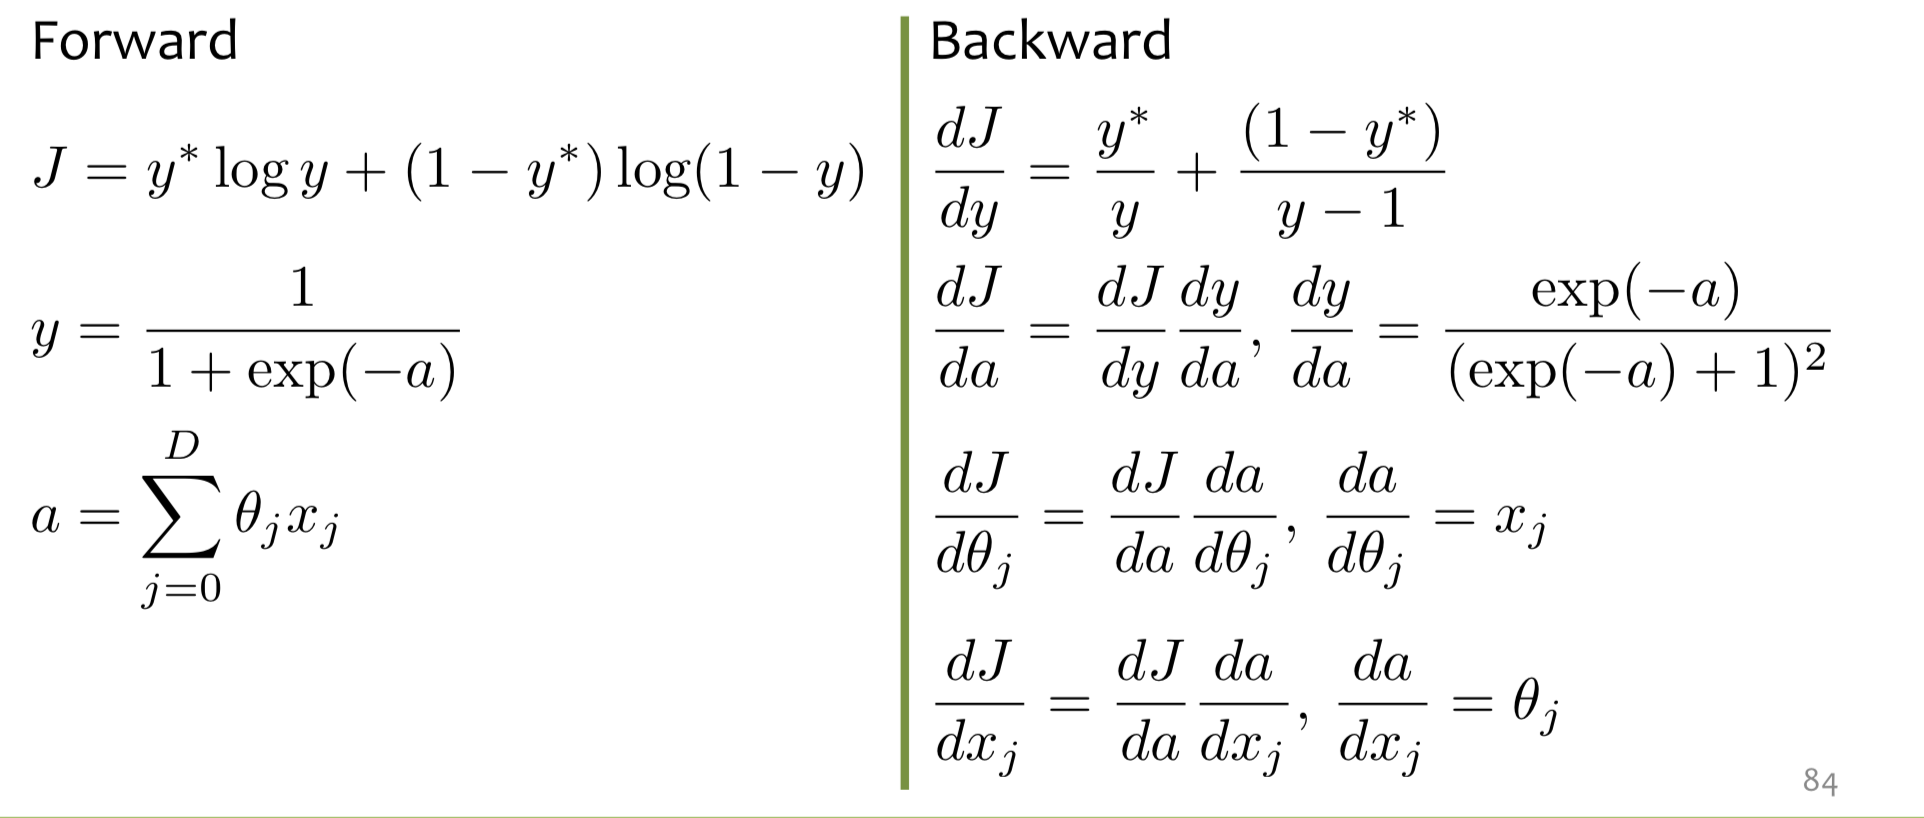
\includegraphics[width=8cm]{figures/backprop.png}
    \caption{Backpropagation for logistic regression}
    \label{fig:backprop}
\end{figure}
    \item Why Backpropagation is fast
    \begin{itemize}
        \item There are only two types of functions in neural network models, i.e., linear and activation functions. 
        \item Derivatives of linear functions are straight forward. We pick activation functions y=f(x) whose derivatives can be expressed as simple functions in y.
        \item During the forward pass, we have computed all relevant variables which would be used in the backward pass.  
    \end{itemize}
\end{itemize}




\section{Training tips}
\label{sec1}
\begin{itemize}
    \item \textbf{Weights initialization} If you initialize all weights to zeros, all hidden units will be identical during the training, which makes it equivalent to "one node" at all layers. This problem is known as "failing to break symmetry". Random initialization fixes this. For random initialization, we usually keep initial parameters small so that activation functions are sensitive at this region. Otherwise you are exposed to vanishing gradient problems. A good example of initialization approach is "He initialization", where weights are random standard normal variables scaled by $2/(\text{dimension of the previous layer})$.  
    \item \textbf{Cut train/validation/test datasets} For relatively small datasets, a 60/20/20 split of train/validation/test sets is usually desirable. However, when you have millions of observations and a sample of 10,000 points is enough for fair performance evaluation purposes, a 98/1/1 split could be better than 60/20/20. 
    \item \textbf{Dev/test sets should be consistent} Sometimes in order to enlarge sample size, you may explore training data whose distribution is not completely the same as that of test data. This is fine as long as you make sure that validation data and test data have the same distribution.
    \item \textbf{Learning curve}
    \begin{itemize}
        \item A large discrepancy between validation and training set errors indicates high variance (overfitting). Possible solutions include enlarging datasets or adding regularizations. 
        \item A large training set error (relative to the base error rate) may indicate high bias (underfitting). Possible solutions include adding complexities to the model architecture.  
        \item If the learning curve is oscillating, it could be that the learning rate is too big/gradients are too large. Clipping gradient norm, reducing learning rate, or a better learning rate decay scheme may help. 
    \end{itemize}

    \item \textbf{Mini batch gradient descent}
    \begin{itemize}
        \item \textbf{Batch gradient descent} Too slow per each iteration. 
        \item \textbf{SGD} Lose the speed up advantage of vectorization.
        \item \textbf{Mini batch gradient descent} 
        \begin{itemize}
            \item Mix of batch gradient descent and SGD.
            \item Better performance for most of the time, especially for large datasets. 
            \item Typical batch sizes include 64, 128, 256, 512. This is also a hyperparameter which can be optimized. (It's better to be the power of 2 due to the way computer memory is layed out)
        \end{itemize}
    \end{itemize}
    
    \item \textbf{Gradients update schemes}
    \begin{itemize}
            \item Momentum gradient descent
    \begin{itemize}
        \item Formula\\
        \begin{align*}
            &V_{dw} = \beta V_{dw} + (1-\beta) dW,~~
            V_{db} = \beta V_{db} + (1-\beta) db\\
            &w:=w-\alpha V_{dw},~~ b:=b-\alpha V_{db}
        \end{align*}
        \item Motivation: When the cost function contour is not spherically symmetric (in high dimensional space), the original gradient descent path may oscillate on the "minor" axis. Momentum helps partially fix this problem by speeding up the movement on the major axis while slowing down the movement on the minor axis. Momentum gradient descent can be thought of as an exponential moving average of the original gradient, which reduces oscillation. 
    \end{itemize}
    \item RMSprop
    \begin{itemize}
        \item Formula
        \begin{align*}
            &S_{dw} = \beta S_{dw} + (1-\beta) \underbrace{dW^2}_{elementwise},~~
            S_{db} = \beta S_{db} + (1-\beta) \underbrace{db^2}_{elementwise} \\
            &w:= w-\alpha\frac{dw}{\sqrt{S_{dw} + \epsilon}},~~
            b:= b-\alpha\frac{db}{\sqrt{S_{db} + \epsilon}}\\
        \end{align*}
        \item Motivation: $w$ is the major axis (where there is a long way from starting point to the minimum) and $b$ is the minor axis (where there is no much difference between starting point and minimum). However, when the cost function contour is a ellipse, the gradient's projection on $b$ is large while the projection on $w$ is small. Thus by dividing ${\sqrt{S_{dw} + \epsilon}}$ or ${\sqrt{S_{db} + \epsilon}}$ we amplify the gradient on $w$ direction. The $\epsilon$ here is just for numerical purposes. (avoid zero denominator)
    \end{itemize}
    \item Adam optimization
    \begin{itemize}
        \item Formula
        \begin{align*}
            &V_{dw} = \beta_1 V_{dw} + (1-\beta_1) dW,~~
            V_{db} = \beta_1 V_{db} + (1-\beta_1) db \xleftarrow{\text{momentum}}\\
            &S_{dw} = \beta_2 S_{dw} + (1-\beta_2) dW^2,~~ 
            S_{db} = \beta_2 S_{db} + (1-\beta_2) db^2
            \xleftarrow{\text{RMSprop}}\\
            &V^{corrected}_{dw} = \frac{V_{dw}}{1-\beta_1^t},~~
            V^{corrected}_{db} = \frac{V_{db}}{1-\beta_1^t}\xleftarrow{\text{bias correction}}\\
            &S^{corrected}_{dw} = \frac{S_{dw}}{1-\beta_2^t},~~
            S^{corrected}_{db} = \frac{S_{db}}{1-\beta_2^t}\xleftarrow{\text{bias correction}}\\
            &w:= w-\alpha\frac{V^{corrected}_{dw}}{\sqrt{S^{corrected}_{dw} + \epsilon}}\\
            &b:= b-\alpha\frac{V^{corrected}_{db}}{\sqrt{S^{corrected}_{db} + \epsilon}}
        \end{align*}
        \item Motivation: This is a combination of momentum and RMSprop algorithms, which is proven to be effective on many deep learning applications. All of momentum, RMSprop, Adam can help learning algorithms get rid of local minimums and saddle points. 
        \item Choice of hyperparameters: 
        \begin{itemize}
            \item $\alpha$: needs to be tune.
            \item $\beta_1$: start with 0.9
            \item $\beta_2$: start with 0.999
            \item $\epsilon$: $10^{-8}$
        \end{itemize}
    \end{itemize}
    \end{itemize}

    \item \textbf{Learning rate decay methods}
    \begin{itemize}
        \item $\alpha = \frac{1}{1+\text{decay rate}*\text{epoch num}} \alpha_0$
        \item $\alpha = 0.95^{\text{epoch num}} \alpha_0$
        \item $\alpha = \frac{k}{epoch num} \alpha_0$
        \item Stepwise functions. (Restricting the number of times that $alpha$ can decay is also a way to realize early stopping)
    \end{itemize}

    \item \textbf{Normalizing features} Make the cost function contour more symmetric so that the gradient descent can proceed faster. 
    \item \textbf{Vanishing/exploding gradients} The gradients can explode/vanish exponentially fast with respect to the number of layers. Proper initialization of weights helps with this problem. For instance, for a single neuron with ReLu activation, we can make $w_i$ be drawn from normal distribution with variance 1/n where n is the number of inputs for this neuron. Clipping gradient norm may also help.

\end{itemize}


\section{How to avoid over-fitting}
    \begin{itemize}
        \item L2 regularization (much more widely used than L1 regularization in neural networks)
        $$
        J(w^{1}, b{1}, ..., w^L, b^L) = \frac{1}{m}\sum_{i=1}^m L(y^{i}, \Hat{y^{i}}) + \frac{\lambda}{2m}\sum_{l=1}^{L}||w^l||_{F}^2
        $$
        where
        \begin{align*}
        ||w^l||_{F}^2 &= \sum_{i=1}^{n[l]}\sum_{j=1}^{n[l-1]}(w^{[l]}_{ij})^2\\
        dw^{[l]} &= \text{(from backprop)} + \frac{\lambda}{m}w^{[l]}\\
        w^{[l]} &= w^{[l]} - \alpha dw^{[l]}\\
        &= \underbrace{(1-\alpha\frac{\lambda}{m})w^{[l]}}_{\text{weight decay}} -\alpha\text{(from backprop)}
        \end{align*}
        \item \textbf{Dropout} Randomly drop a certain fraction of nodes at each layer. Multiply the weights of the remaining layer by (1/fraction remained). It helps prevent over-fitting because the dropout process prevents the situation that one node is being relied on too much. When weights are more spread out on different nodes, the Frobenius norm of the weight matrix decreases. Dropout is not applied on the test set. 
        \item \textbf{Data Augmentation} Flip, rotate, zooming in, etc.
        \item \textbf{Early stopping} 
        \begin{itemize}
            \item \textbf{Advantage} You only have to go through gradient descent process once without trying lots of different values for $\lambda$.
            \item \textbf{Disadvantage} The task of minimizing cost function and the task of regularization are not orthogonal. (The algorithm learns better when these two tasks are well separated) 
        \end{itemize}
        \item Reduce the architecture complexity to make it more generalizable. 
    \end{itemize}
    

\section{Hyperparameter tuning}
\begin{itemize}
    \item Tuning Process
    \begin{itemize}
        \item Hyperparameters\\
1. Learning rate $\alpha$\\
2. Number of hidden units, mini-batch size, hyperparameters for gradient descent with momentum $\beta$\\
\tab a. Mini-batch size is usually the power of 2\\
\tab b. $\beta$ is usually 0.9\\
3. Number of layers, learning rate decay, hyperparamters for Adam optimization algorithm $\beta_{1}$ $\beta_{2}$ $\epsilon$\\
\tab a. $\beta_{1}$ is usually 0.9\\
\tab b. $\beta_{2}$ is usually 0.999\\
\tab c. $\epsilon$ is usually $10^{-8}$
        \item Tuning tricks\\
1. Pick hyperparameters at random from coarse to fine.\\
\tab a. Do not use grid because hyper parameters are not equally important.\\
\tab b. Zoom in to a smaller region of the hyperparameters that works well and then sample more density within this area.\\
2. Choose appropriate scale for hyperparameters.\\
\tab a. Learning rate $\alpha$: $10^{-4}$, $10^{-3}$, $10^{-2}$, $10^{-1}$, $10^{0}$\\
\tab b. Hyperparameters for exponentially weighted averages $\beta$: $1 - 10^{-4}$, $1 - 10^{-3}$, $1 - 10^{-2}$, $1 - 10^{-1}$
        \item Tuning in practice\\
1. Re-test hyperparameters occasionally\\
2. Two ways of searching for hyperparameters\\
\tab a. Train one model at a time\\
\tab b. Train many different models in parallel\\
    \end{itemize}
    \item Batch Normalization
    \begin{itemize}
        \item Normalize activations in a network\\
1. Normalize inputs to speed up training\\
\tab a. Turn the contours of the learning problem from something elongated to something more round\\
\tab b. Easier for an algorithm like gradient descent to optimize. \\
2. Normalize each layer before the activation function \\
\tab a.  Get $z_{i,norm}$ by subtracting off the mean and dividing by the standard deviation\\ 
\tab b. $\widetilde{z} = \gamma * z_{i,norm} + \beta$\\ 
\tab c. $\gamma$ and $\beta$ are learnable parameters of the model
        \item Fit batch norm into neural network\\
$x \xrightarrow{w^{[1]} b^{[1]}}z^{[1]} \xrightarrow[Batch Norm]{\beta^{[1]} \gamma^{[1]}}\widetilde{z}^{[1]}\xrightarrow{}a^{[1]}=g(z^{[1]})\xrightarrow{w^{[2]} b^{[2]}}z^{[2]}$...\\

Parameters: $w^{[1]}, b^{[1]}, \beta^{[1]}, \gamma^{[1]},$...$w^{[L]}, b^{[L]}, \beta^{[L]}, \gamma^{[L]},$\\
$\beta^{[l]} = \beta^{[l]} - \alpha*d\beta^{[l]}$
        \item Implement gradient descent\\
For t = 1, 2, ..., num of mini-batches:\\
\tab Compute forward propagation on $X^{[t]}$\\
\tab\tab In each hidden layer, use batch norm to replace $z^{[l]}$ with $\widetilde{z}^{[l]}$\\
\tab Use back propagation to compute $dw^{[l]}, d\beta^{[l]}, d\gamma^{[l]}$\\
\tab Update parameters:\\
\tab\tab$w^{[l]} = w^{[l]} - \alpha*dw^{[l]}$\\
\tab\tab$\beta^{[l]} = \beta^{[l]} - \alpha*d\beta^{[l]}$\\
\tab\tab$\gamma^{[l]} = \gamma^{[l]} - \alpha*d\gamma^{[l]}$\\
Work with momentum, RMS, Adam...\\
        \item Why does batch norm work\\
1. By normalizing all the features, input X takes on a similar range of values that can speed up learning\\
2. Batch norm makes weights deeper in the network more robust to changes to weights in earlier layers of the neural network\\
3. Batch norm has slightly regulation effect. 
        \item Batch norm at a test time\\
Estimate mean and variance using an exponentially weighted average where the average is across the mini batches.\\
\tab a. For layer l, keep track of sample mean and variance for each mini batch when training on them $\mu^{\{1\}[l]}, \mu^{\{2\}[l]},...,\mu^{\{M\}[l]}, \sigma^{2\{1\}[l]}, \sigma^{2\{2\}[l]},...,\sigma^{2\{M\}[l]}$\\
\tab b. Use the exponentially weighted average mean $\mu$ and variance $\sigma^{2}$ to get $z_{norm} = \frac{(z-\mu)}{\sqrt{\sigma^{2}+\epsilon}}$
    \end{itemize}
    \item{Multi-class classification} 
    \begin{itemize}
        \item Softmax regression\\
1. In multi-class classification problem, the output layer is softmax layer to generate probabilities.\\
2. Activation function for softmax layer: $a = g(z) = \frac{z}{\sum(z)}$\\
3. Softmax layer with no hidden layers gives linear boundaries.
        \item Train softmax layer\\
1. Loss function: \\
\tab a. $\hat{y} = a^{[L]} = g(z^{[L]})$\\
\tab b. $Loss(\hat{y},y) = -\sum_{i=1}^{C}y_{i}log(\hat{y}_{i})$\\
2. Back propogation:\\
\tab a. $dz^{[L]} = \hat{y} - y$\\
    \end{itemize}
    \item{Introduction to program frameworks} 
    \begin{itemize}
        \item Tensorflow broad structure\\
1. start: \\
\tab import numpy as np\\
\tab import tensorflow as tf\\
2. define variable:\\
\tab coeff = np.array([[1.],[-10.],[25.]])\\
\tab w = tf.Variable(0, dtype = tf.float32)\\
\tab x = tf.placeholder(tf.float32, [3,1])\\
\tab cost = x[0][0]*w**2 + x[1][0]*w + x[2][0]\\
3. train:\\
\tab train = tf.train.GradientDescentOptimizer(0.01).minimize(cost)\\
\tab init = tf.global\_variables\_initializer()\\
\tab with tf.Session() as session:\\
\tab\tab session.run(init)\\
\tab\tab print(session.run(w))\\
\tab for i in range(1000):\\
\tab\tab session.run(train, feed\_dict={x: coeff})\\
\tab print(session.run(w))\\
    \end{itemize}
\end{itemize}    
    

\section{Convolution neural networks}
\begin{itemize}
    \item \textbf{Step by Step}\\
    Input matrix $\xrightarrow{convolution}$ feature maps $\xrightarrow{activation function}$activated feature maps\\ $\xrightarrow{pooling}$pooling layers$\xrightarrow{...}$...
    \item \textbf{filter/kernel/feature detector} You will slide the filter over the original input matrix to compute a matrix called "convolved feature/activation map/feature map".
    \item \textbf{convolved feature/activation map/feature map} See \ref{fig:cnn1}.
    \item \textbf{Attributes of feature map} 
    \begin{itemize}
        \item \textit{Depth} The number of filters we used for convolution operation. If depth=n, the feature map will be n stacked matrices.  
        \item \textit{Stride} The number of "cell" (e.g., pixels) by which we slide the filter over the input matrix. 
        \item \textit{Zero-padding} Whether to pad the input matrix with zeros around the boarder. Zero padding allows us to control the size of the feature map.  
    \end{itemize}
    \item \textbf{Pooling/Sub-sampling}:For example, in case of max pooling, we define a spatial neighborhood and take the largest element from the activated(e.g., rectified) feature map within this neighborhood. We can also do average pooling, etc. Pooling is a method to reduce dimensionality while retaining the most important information.
\end{itemize}
    \begin{figure}[h]
        \centering
        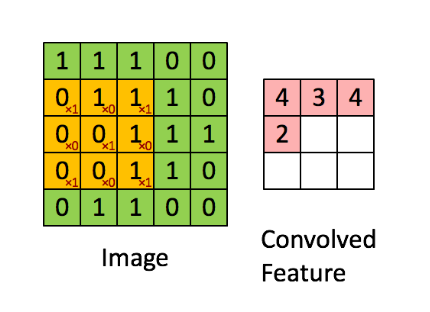
\includegraphics[width=5cm]{figures/CNN1.png}
        \caption{The convolution operation. The green matrix is the original input matrix. The yellow matrix is the filter. The pink output is the convolved feature.}
        \label{fig:cnn1}
    \end{figure}


\section{Interpretation}
\begin{itemize}
    \item \textbf{Neural networks and brain}  "A single neuron in the brain is an incredibly complex machine that even today we don’t understand. A single “neuron” in a neural network is an incredibly simple mathematical function that captures a minuscule fraction of the complexity of a biological neuron. So to say neural networks mimic the brain, that is true at the level of loose inspiration, but really artificial neural networks are nothing like what the biological brain does." --Andrew Ng
    \item \textbf{Why CNN} Convolution operation is a way to extract low-level features from the input. When the stride is larger than 1, it has down-sampling effect. (The activation map now has lower dimensions than the input) It's sort of like PCA, where we use a low dimensional representation to capture the most important characteristics of the original input matrix. Convolution is also a way to capture local dependencies. 
\end{itemize}

%%%%%%%%%%%%%%%%%%%%%%%%%%%%%%%%%%%%%%%%%%%%%%%%%%%%%%%%
%% Sample table                                        %
%% Source: www1.maths.leeds.ac.uk/latex/TableHelp1.pdf %
%%%%%%%%%%%%%%%%%%%%%%%%%%%%%%%%%%%%%%%%%%%%%%%%%%%%%%%%
%\begin{table}[ht]
%\caption{Sample table} % title of Table
%\centering % used for centering table
%\begin{tabular}{c c c c}
%% centered columns (4 columns)
%\hline\hline %inserts double horizontal lines
%S. No. & Column\#1 & Column\#2 & Column\#3 \\ [0.5ex]
%% inserts table
%%heading
%\hline % inserts single horizontal line
%1 & 50 & 837 & 970 \\
%2 & 47 & 877 & 230 \\
%3 & 31 & 25 & 415 \\
%4 & 35 & 144 & 2356 \\
%5 & 45 & 300 & 556 \\ [1ex] % [1ex] adds vertical space
%\hline %inserts single line
%\end{tabular}
%\label{table:nonlin} % is used to refer this table in the text
%\end{table}


